\documentclass[border=4pt]{standalone}
\usepackage{tikz}
\usepackage{pgfplots}
\pgfplotsset{compat=1.18}
\usepgfplotslibrary{statistics}
\usetikzlibrary{patterns, arrows.meta, positioning, calc}
\usepackage{amsmath, amssymb}
\usepackage{bm}

% ===== Color palette (IEEE-style muted, Ours = saturated) =====
\definecolor{cCNN}{HTML}{A8B8CC}     % muted blue-gray
\definecolor{cEPI}{HTML}{B8C8A8}     % muted olive
\definecolor{cATT}{HTML}{E8C28A}     % muted gold
\definecolor{cDM}{HTML}{C4A8C8}      % muted mauve
\definecolor{cOurs}{HTML}{C0392B}    % deep red (highlight)
\definecolor{cOursDark}{HTML}{7B241C}

\begin{document}
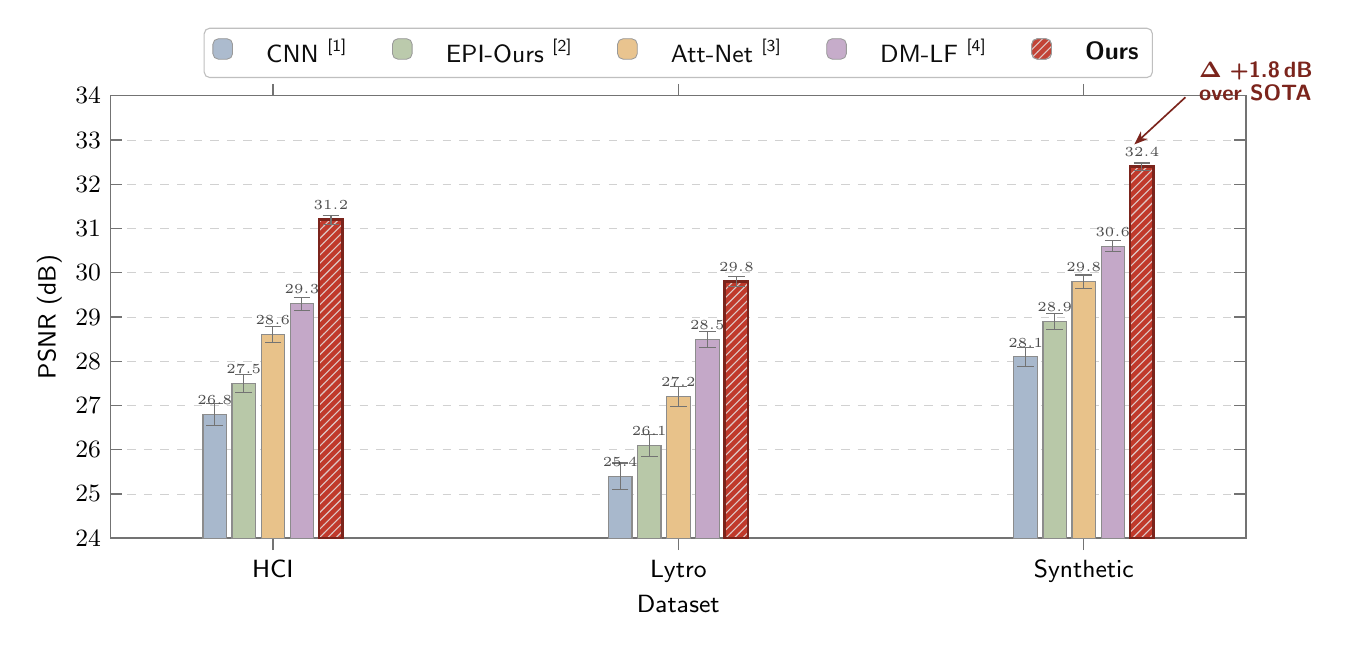
\begin{tikzpicture}
\begin{axis}[
    ybar,
    bar width=8.5pt,
    width=16cm,
    height=7.2cm,
    enlarge x limits=0.20,
    symbolic x coords={HCI, Lytro, Synthetic},
    xtick=data,
    xlabel={Dataset},
    ylabel={PSNR (dB)},
    ymin=24, ymax=34,
    ytick={24,25,26,27,28,29,30,31,32,33,34},
    ymajorgrids=true,
    grid style={dashed, black!18, line width=0.3pt},
    axis line style={black!55, line width=0.5pt},
    tick style={black!55, line width=0.5pt},
    tick label style={font=\sffamily\small},
    label style={font=\sffamily\small},
    xlabel style={yshift=2pt},
    ylabel style={yshift=-2pt},
    legend style={
        at={(0.5,1.04)},
        anchor=south,
        legend columns=5,
        font=\sffamily\small,
        draw=black!25,
        fill=white,
        fill opacity=0.95,
        rounded corners=2pt,
        column sep=10pt,
        /tikz/every even column/.append style={column sep=14pt},
    },
    legend image code/.code={
        \draw[#1, draw=black!40, line width=0.3pt]
            (0cm,-0.08cm) rectangle (0.25cm,0.18cm);
    },
    legend cell align={left},
    every axis plot/.append style={
        draw=black!45,
        line width=0.4pt,
    },
    nodes near coords,
    nodes near coords style={
        font=\sffamily\tiny,
        text=black!70,
        anchor=south,
        /pgf/number format/fixed,
        /pgf/number format/precision=1,
    },
    error bars/y dir=both,
    error bars/y explicit,
    error bars/error bar style={black!55, line width=0.4pt},
    error bars/error mark options={
        rotate=90,
        mark size=3pt,
        line width=0.4pt,
    },
    visualization depends on=y value \as \yval,
]

% ----- Method 1: CNN baseline -----
\addplot[fill=cCNN, draw=black!45, line width=0.4pt]
    coordinates {
    (HCI,26.8) +- (0,0.25)
    (Lytro,25.4) +- (0,0.30)
    (Synthetic,28.1) +- (0,0.22)
    };

% ----- Method 2: EPI-based -----
\addplot[fill=cEPI, draw=black!45, line width=0.4pt]
    coordinates {
    (HCI,27.5) +- (0,0.20)
    (Lytro,26.1) +- (0,0.25)
    (Synthetic,28.9) +- (0,0.18)
    };

% ----- Method 3: Attention Network -----
\addplot[fill=cATT, draw=black!45, line width=0.4pt]
    coordinates {
    (HCI,28.6) +- (0,0.18)
    (Lytro,27.2) +- (0,0.22)
    (Synthetic,29.8) +- (0,0.15)
    };

% ----- Method 4: Diffusion Model -----
\addplot[fill=cDM, draw=black!45, line width=0.4pt]
    coordinates {
    (HCI,29.3) +- (0,0.15)
    (Lytro,28.5) +- (0,0.18)
    (Synthetic,30.6) +- (0,0.12)
    };

% ----- Ours (highlighted: deep red + bold black edge + pattern) -----
\addplot[
    fill=cOurs,
    draw=cOursDark,
    line width=0.9pt,
    postaction={
        pattern=north east lines,
        pattern color=white!75!cOursDark,
    },
]
    coordinates {
    (HCI,31.2) +- (0,0.10)
    (Lytro,29.8) +- (0,0.12)
    (Synthetic,32.4) +- (0,0.08)
    };

\legend{
    {CNN~\textsuperscript{[1]}},
    {EPI-Ours~\textsuperscript{[2]}},
    {Att-Net~\textsuperscript{[3]}},
    {DM-LF~\textsuperscript{[4]}},
    {\textbf{Ours}},
}

\end{axis}

% ----- Annotation: best performer callout -----
% Positioned relative to the axis area to emphasize "Ours"
\node[font=\sffamily\footnotesize\bfseries, text=cOursDark,
      anchor=west, align=left]
      at (13.7,5.8) {$\bm{\Delta}$ +1.8\,dB\\[-1pt]over SOTA};
\draw[-{Stealth[length=5pt]}, line width=0.6pt, cOursDark]
      (13.65,5.6) -- (13.0,5.0);

\end{tikzpicture}
\end{document}